\subsection{Data List Interface}

The data list interface presents the records retrieved from the \texttt{GAME} table together with related information from the \texttt{DEVELOPER} table. It is implemented in the React component \texttt{GameList.jsx} and is the central screen of the application: it integrates a data list, a search panel powered by the stored procedure \texttt{GetGamesByGenreAndPrice} from Section~5.3, and inline action buttons that reuse the CRUD stored procedures from Section~5.1. This consolidated design keeps the user workflow consistent because the same screen that displays the list also lets the user select a row and immediately add, update, or delete the record.

\subsubsection{Interface Overview}

When the page loads, three asynchronous calls are issued in parallel: \texttt{GET /api/games} to retrieve the full list of games, \texttt{GET /api/genres} to populate the genre dropdown, and \texttt{GET /api/developers} to populate the developer dropdown used in the modal form. The retrieved games are rendered as rows in an HTML table with the columns \textit{ID}, \textit{Game Title}, \textit{Price (USD)}, \textit{Release Date}, and \textit{Developer}. A row becomes the \emph{selected row} when the user clicks on it and is highlighted with a colored left border; the selected row is the target of the \textit{Edit Selected} and \textit{Delete Selected} actions.

\begin{table}[H]
\centering
\caption{Main features of the data list interface}
\label{tab:gamelist-features}
\begin{tabular}{|l|p{9cm}|}
\hline
\textbf{Feature} & \textbf{Description} \\ \hline
List display & Loads all games via \texttt{GET /api/games} and renders them in a table with five columns. \\ \hline
Refresh & A \textit{Refresh} button re-issues the games query to reflect any change made by another user. \\ \hline
Search by genre and max price & Calls the stored procedure \texttt{GetGamesByGenreAndPrice} via \texttt{POST /api/search}, returning only games that match both filters. \\ \hline
Clear search & Restores the full list by re-issuing \texttt{GET /api/games}. \\ \hline
Sortable columns & Each header column supports ascending/descending sort on the client side (see Section~\ref{subsec:sort-detail}). \\ \hline
Add a new game & Opens a modal form bound to \texttt{POST /api/games} (\texttt{sp\_InsertGame}). \\ \hline
Edit selected game & Opens the same modal in edit mode and submits via \texttt{PUT /api/games/:id} (\texttt{sp\_UpdateGame}). \\ \hline
Delete selected game & Confirms the user's intent and issues \texttt{DELETE /api/games/:id} (\texttt{sp\_DeleteGame}). \\ \hline
Inline messages & A red banner shows error messages and a green banner shows success messages; both can be dismissed manually or auto-hide after three seconds. \\ \hline
\end{tabular}
\end{table}

\subsubsection{Search and Filtering}

The search panel contains a \textit{Genre} dropdown populated from the \texttt{GENRE} table and a \textit{Max Price (USD)} numeric input. When the user clicks \textit{Search}, the frontend validates that a genre is selected and that the price is a non-negative number. If validation fails, the request is not sent and an inline error message is displayed. Otherwise the frontend sends a JSON body \texttt{\{ genre, maxPrice \}} to \texttt{POST /api/search}, and the backend forwards the parameters to the stored procedure \texttt{GetGamesByGenreAndPrice}. The backend returns the result rows, which replace the current list. If the procedure returns an empty result, the interface displays the friendly message \textit{``No games found for genre X under Y USD''} so that the user can adjust the filter without confusion.

\subsubsection{Sorting}\label{subsec:sort-detail}

In addition to the database-level filtering provided by the stored procedure, the interface supports client-side sorting on every column. When the user clicks a column header, the games array stored in the React state is sorted by the corresponding field. Successive clicks on the same header toggle between ascending and descending order. Sorting is applied locally so that re-sorting a list of fewer than a few hundred rows is instantaneous and does not require a round trip to the database.

\subsubsection{Update and Delete Directly from the List}

The two operations \emph{update} and \emph{delete} are deliberately performed against the row currently selected in the list. To update, the user clicks a row to mark it as the selected row, then clicks \textit{Edit Selected}. The modal form opens pre-filled with the selected game's title, base price, and release date; when the user confirms, the frontend issues \texttt{PUT /api/games/:id}, which calls \texttt{sp\_UpdateGame} on the database side. To delete, the user clicks a row, then clicks \textit{Delete Selected}; a JavaScript \texttt{window.confirm} dialog asks for confirmation, and on agreement the frontend issues \texttt{DELETE /api/games/:id}, which calls \texttt{sp\_DeleteGame}. Both operations invalidate the list and trigger an automatic re-fetch so that the table always reflects the latest state of the database.

\subsubsection{Input Validation and Error Handling}

The interface enforces validation at two levels. On the frontend, before any HTTP request is sent, it checks for empty titles, non-numeric or negative prices, missing release dates, and missing developer selection (for the insert form). On the backend, the stored procedures \texttt{sp\_InsertGame}, \texttt{sp\_UpdateGame}, and \texttt{sp\_DeleteGame} perform the authoritative validation, including foreign key existence checks and the rule that a game already owned in a player's library cannot be deleted. Whenever a stored procedure raises a \texttt{SIGNAL SQLSTATE '45000'} error, the backend forwards the original message to the frontend, where it is displayed in the red error banner. This guarantees that the user always sees a clear, specific error message rather than a generic ``request failed'' notice.

\begin{table}[H]
\centering
\caption{Examples of validation and error handling on the data list interface}
\label{tab:gamelist-validation}
\begin{tabular}{|p{4.5cm}|p{4cm}|p{5cm}|}
\hline
\textbf{User action} & \textbf{Validation layer} & \textbf{Resulting message} \\ \hline
Click \textit{Edit Selected} without selecting a row & Frontend & ``Please select a game first.'' \\ \hline
Submit the modal with an empty title & Frontend & ``Game title cannot be empty.'' \\ \hline
Submit the modal with negative price & Frontend & ``Price must be a positive number.'' \\ \hline
Insert a game whose \texttt{developer\_id} does not exist & Backend (\texttt{sp\_InsertGame}) & Original SQL error forwarded to the banner. \\ \hline
Delete a game that is already owned by a player & Backend (\texttt{sp\_DeleteGame}) & ``Cannot delete game that is already owned by players.'' \\ \hline
\end{tabular}
\end{table}

\subsubsection{Execution Result}

The screenshots below illustrate the data list interface in operation. Figure~\ref{fig:data-list-interface} shows the default view after the page loads with the full list of games, the row currently selected by the user (highlighted in red), the action buttons \textit{Add New Game}, \textit{Edit Selected}, and \textit{Delete Selected}, and the \textit{Refresh} button. Figure~\ref{fig:data-list-search-result} shows the result of calling the stored procedure \texttt{GetGamesByGenreAndPrice} with a filter that returns no matching record, including the friendly empty-state message produced by the frontend. Figure~\ref{fig:data-list-edit-modal} shows the modal that opens when the user clicks \textit{Edit Selected}. Figure~\ref{fig:data-list-delete-confirm} shows the browser confirmation dialog displayed before \texttt{sp\_DeleteGame} is called. Figure~\ref{fig:data-list-error-select} and Figure~\ref{fig:data-list-error-addmodal} demonstrate the two main error scenarios: clicking \textit{Edit Selected} without selecting a row, and submitting the \textit{Add New Game} modal with an empty title.

\begin{figure}[H]
    \centering
    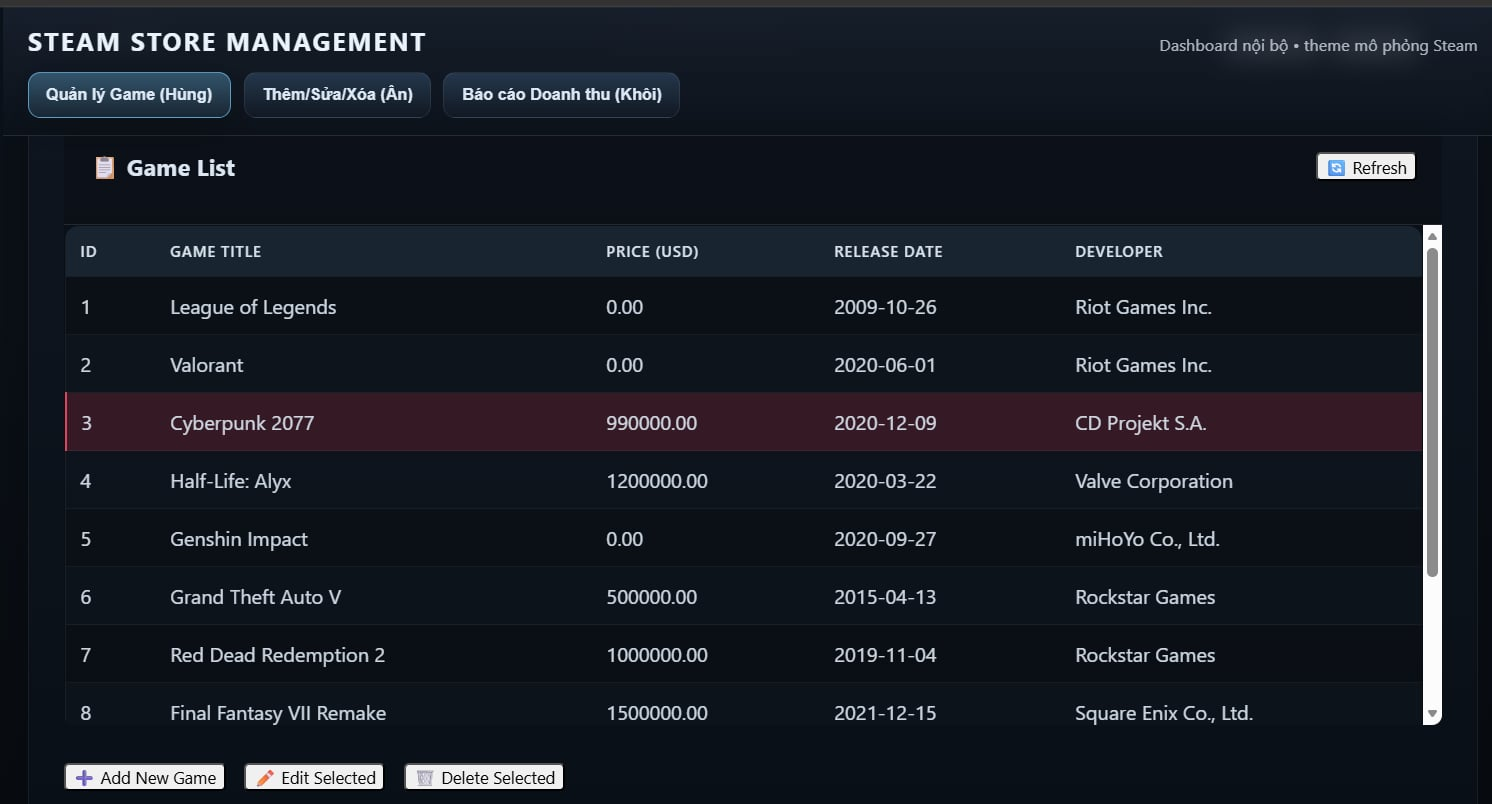
\includegraphics[width=0.95\linewidth]{graphics/data_list_interface.jpg}
    \caption{Default view of the data list interface, with one game row selected}
    \label{fig:data-list-interface}
\end{figure}

\begin{figure}[H]
    \centering
    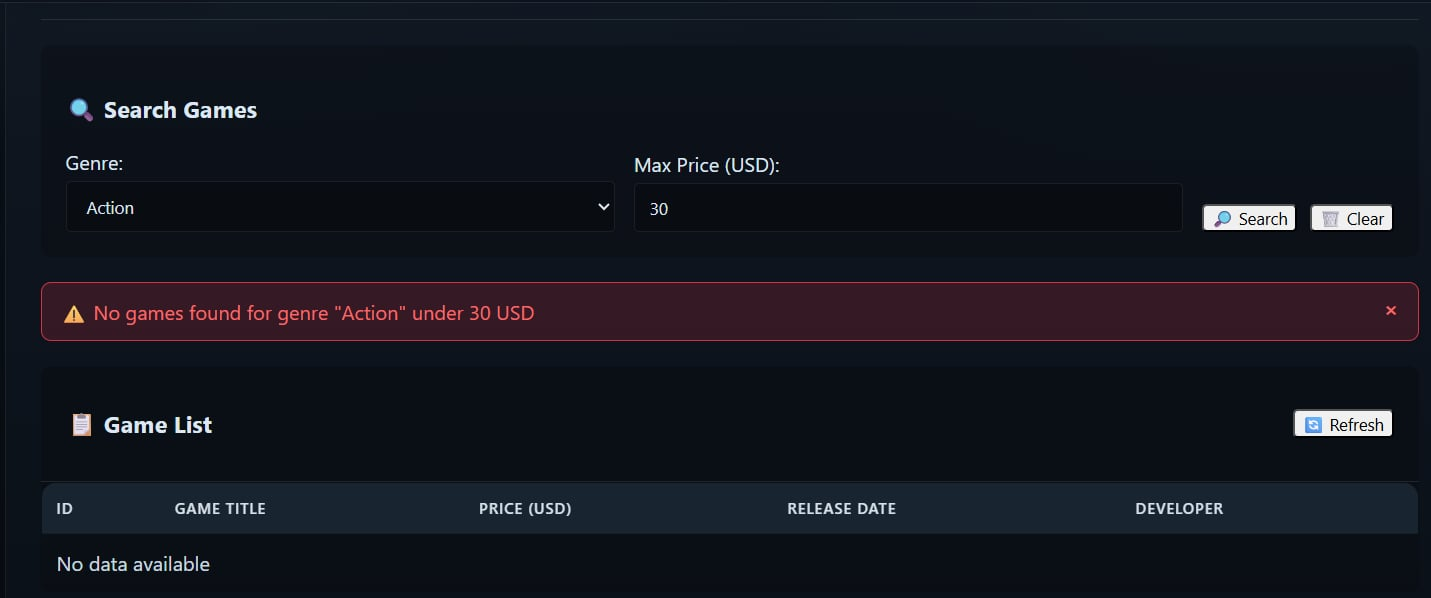
\includegraphics[width=0.95\linewidth]{graphics/data_list_search_result.jpg}
    \caption{Filtered list after invoking \texttt{GetGamesByGenreAndPrice}, showing the friendly empty-result message}
    \label{fig:data-list-search-result}
\end{figure}

\begin{figure}[H]
    \centering
    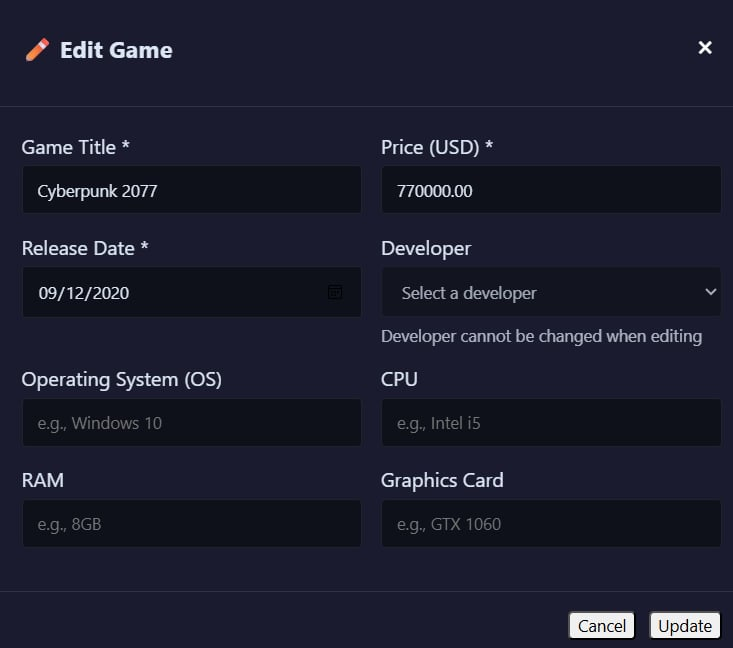
\includegraphics[width=0.7\linewidth]{graphics/data_list_edit_modal.jpg}
    \caption{Modal form opened by clicking \textit{Edit Selected}, pre-filled with the selected game's data}
    \label{fig:data-list-edit-modal}
\end{figure}

\begin{figure}[H]
    \centering
    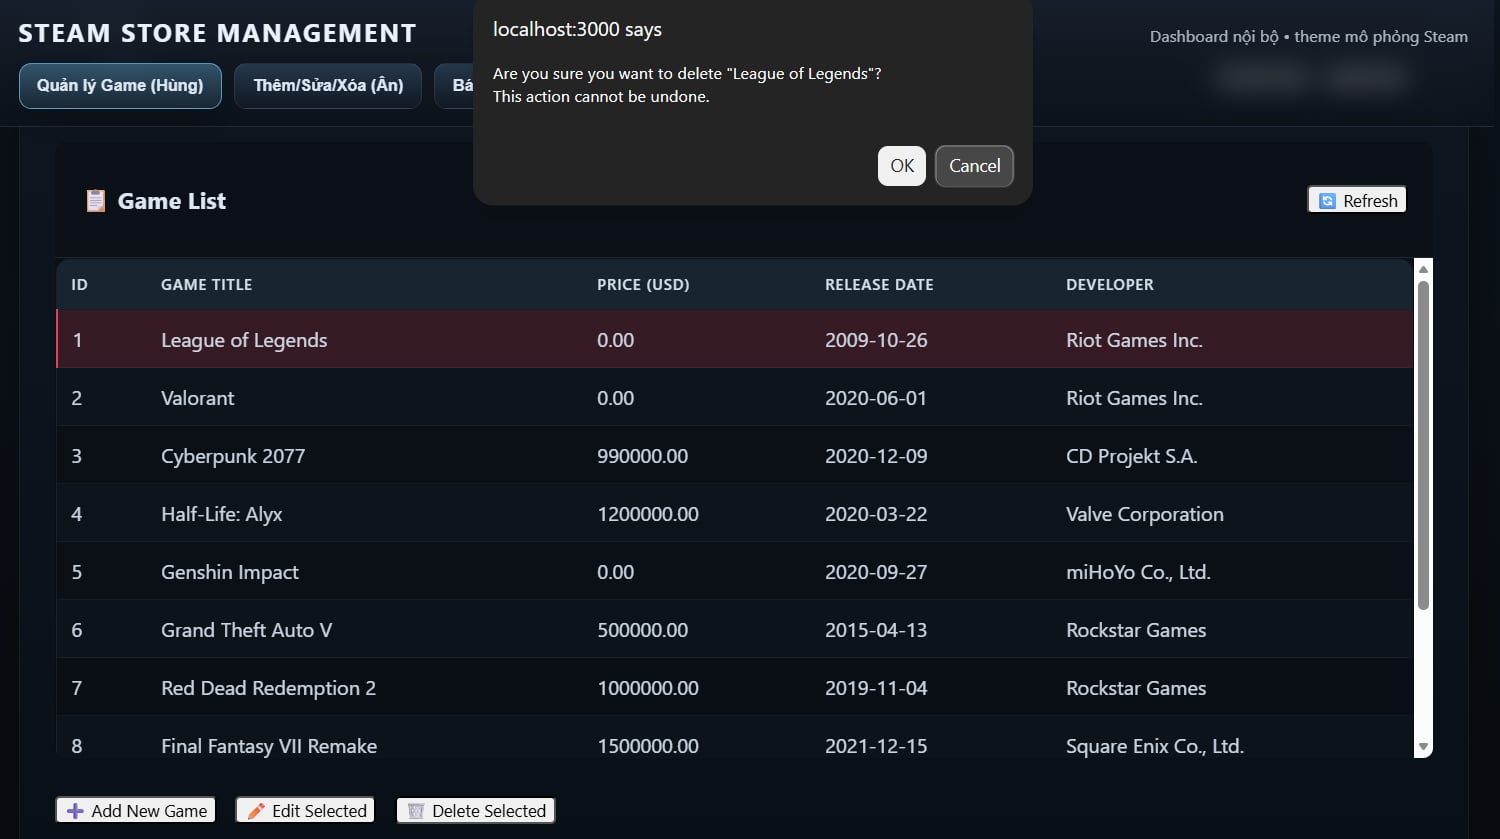
\includegraphics[width=0.95\linewidth]{graphics/data_list_delete_confirm.jpg}
    \caption{Browser confirmation dialog displayed before deleting the selected game}
    \label{fig:data-list-delete-confirm}
\end{figure}

\begin{figure}[H]
    \centering
    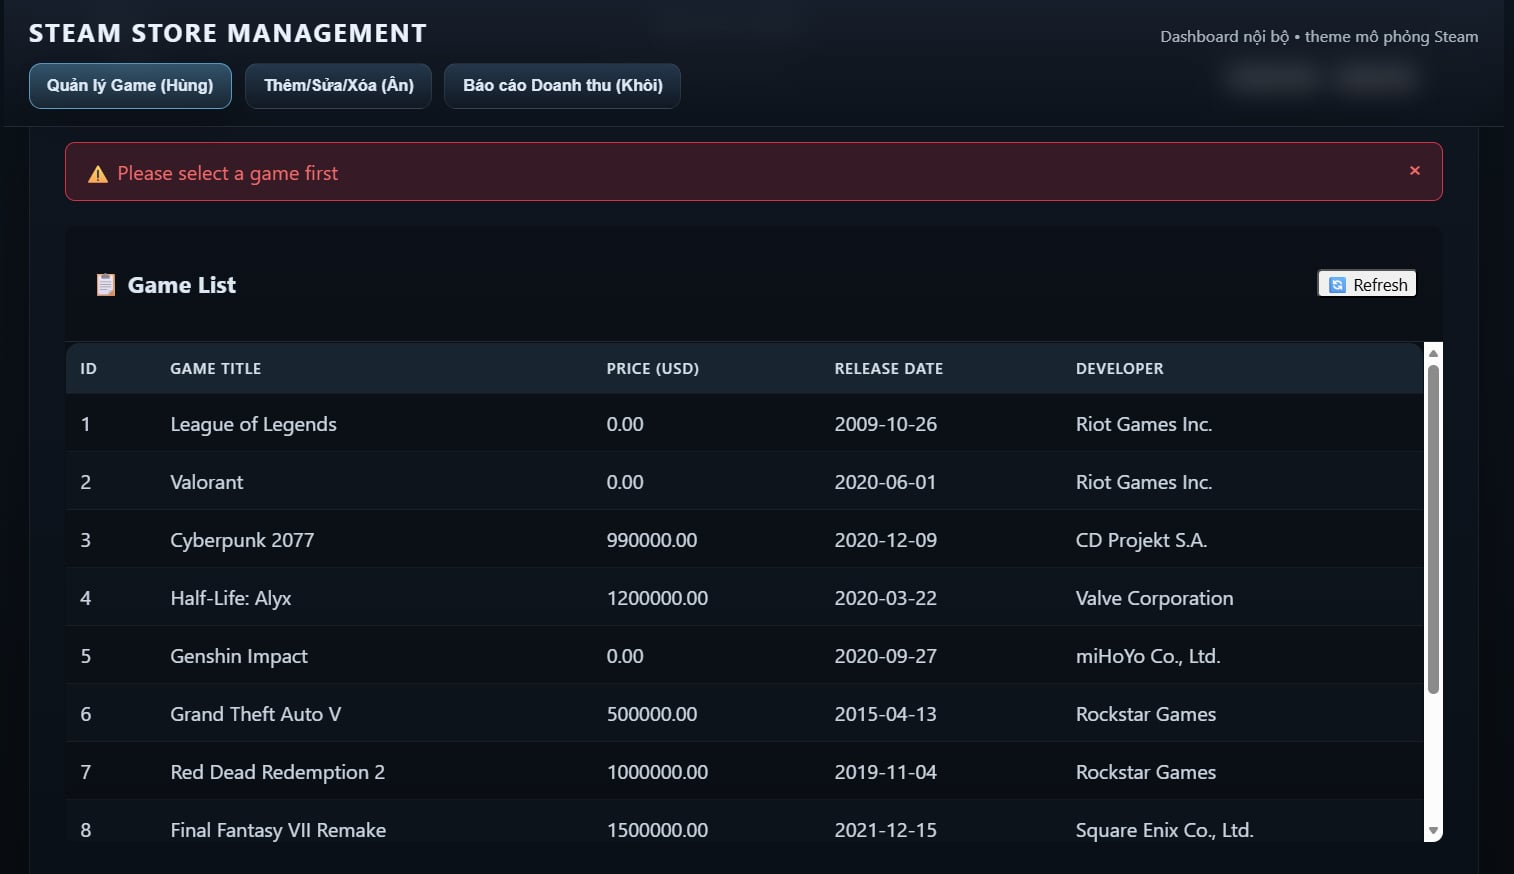
\includegraphics[width=0.95\linewidth]{graphics/data_list_error_select.jpg}
    \caption{Frontend validation error when clicking \textit{Edit Selected} with no row selected}
    \label{fig:data-list-error-select}
\end{figure}

\begin{figure}[H]
    \centering
    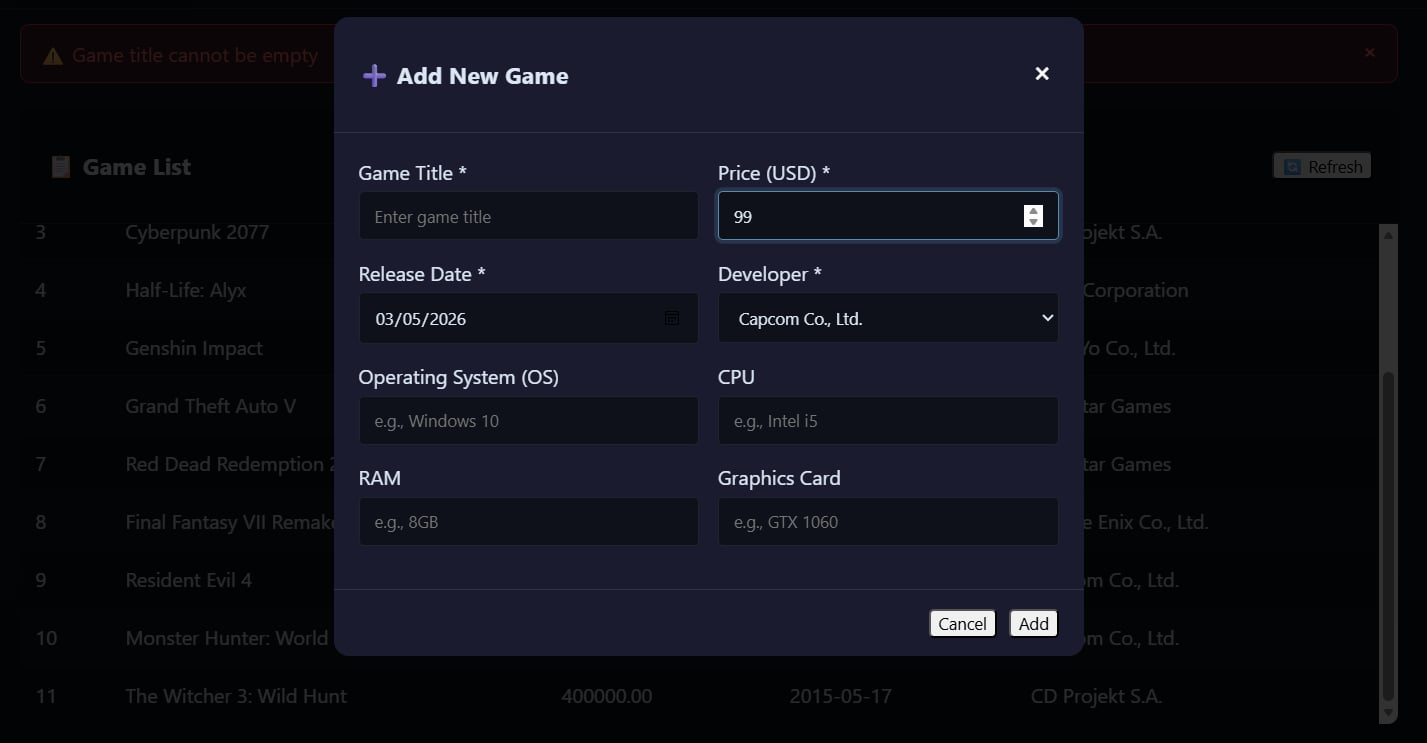
\includegraphics[width=0.95\linewidth]{graphics/data_list_error_addmodal.jpg}
    \caption{Frontend validation error when submitting the \textit{Add New Game} modal with an empty title}
    \label{fig:data-list-error-addmodal}
\end{figure}
